% This is part of Un soupçon de mathématique sans être agressif pour autant
% Copyright (c) 2015
%   Laurent Claessens
% See the file fdl-1.3.txt for copying conditions.

% This is part of Un soupçon de mathématique sans être agressif pour autant
% Copyright (c) 2015
%   Laurent Claessens
% See the file fdl-1.3.txt for copying conditions.

%--------------------------------------------------------------------------------------------------------------------------- 
\subsection*{Activité : Sur une pyramide}
%---------------------------------------------------------------------------------------------------------------------------

Recopier et compléter le patron suivant de pyramide.

\begin{center}
   \input{Fig_PIMUooMLLYDU.pstricks}
\end{center}


Quelle est la distance à parcourir \emph{sur la pyramide} pour aller de \( P\) à \( N\) ?




%+++++++++++++++++++++++++++++++++++++++++++++++++++++++++++++++++++++++++++++++++++++++++++++++++++++++++++++++++++++++++++ 
\section{Pyramide}
%+++++++++++++++++++++++++++++++++++++++++++++++++++++++++++++++++++++++++++++++++++++++++++++++++++++++++++++++++++++++++++

\begin{definition}[\cite{NRHooXFvgpp4}]
    Une \defe{pyramide}{pyramide} est un solide dont :
    \begin{itemize}
        \item 
            une face est un polygone appelée la \defe{base}{base!d'une pyramide} de la pyramide ;
\item
les autres faces, appelées faces latérales, sont des triangles qui ont un sommet commun, appelé le sommet de la pyramide.
    \end{itemize}
\end{definition}


\begin{definition}[\cite{NRHooXFvgpp4}]
    \begin{itemize}
        \item 
La hauteur d'une pyramide est le segment issu de son sommet et perpendiculaire à la base.
\item
Une arête latérale est un segment joignant les sommets de la base au sommet de la pyramide.
    \end{itemize}
\end{definition}

% This is part of Un soupçon de mathématique sans être agressif pour autant
% Copyright (c) 2015
%   Laurent Claessens
% See the file fdl-1.3.txt for copying conditions.

%--------------------------------------------------------------------------------------------------------------------------- 
\subsection*{Activité : Patron d'un cône}
%---------------------------------------------------------------------------------------------------------------------------

Ceci est un petit cône en papier :
\begin{center}
    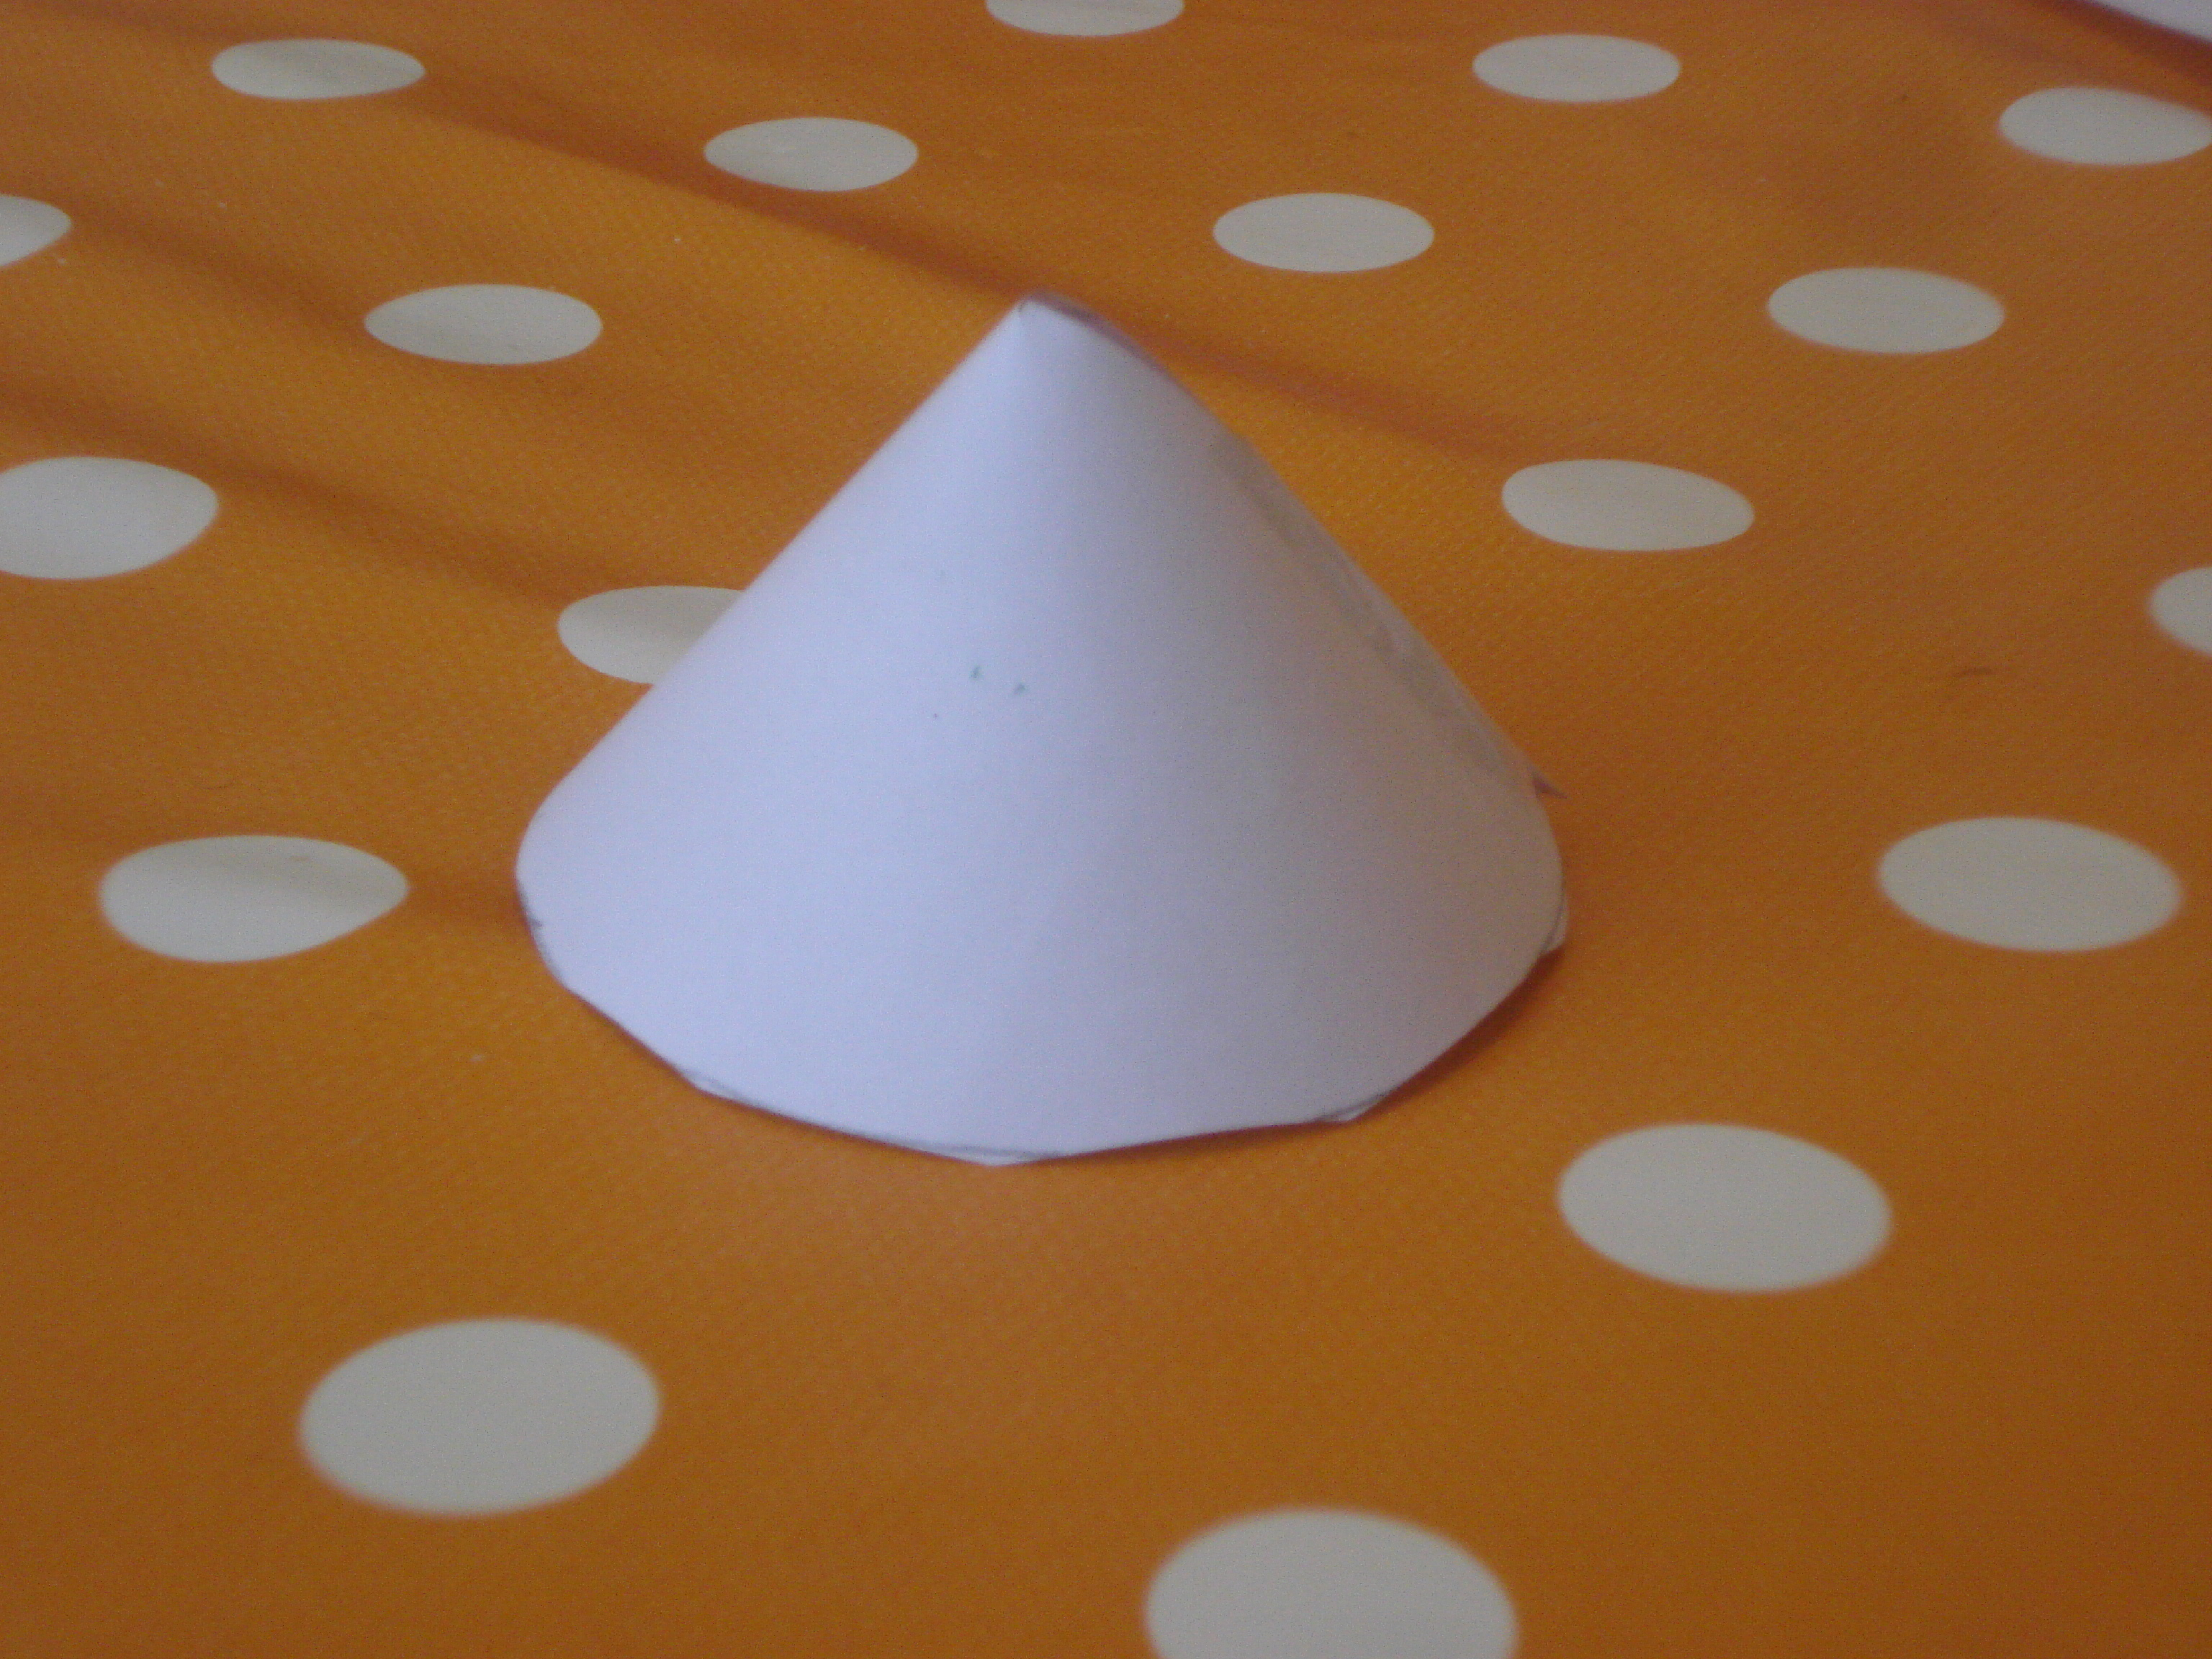
\includegraphics[width=5cm]{cone_papier.pdf}
\end{center}

\begin{enumerate}
    \item
        Comment réalise-t-on ce pliage ? Le faire.
    \item
        Comment découper le papier pour obtenir au bout du compte un cône dont le rayon de la base soit \SI{3}{\centi\meter} et la hauteur \SI{4}{\centi\meter} ?
\end{enumerate}


%+++++++++++++++++++++++++++++++++++++++++++++++++++++++++++++++++++++++++++++++++++++++++++++++++++++++++++++++++++++++++++ 
\section{Cône de révolution}
%+++++++++++++++++++++++++++++++++++++++++++++++++++++++++++++++++++++++++++++++++++++++++++++++++++++++++++++++++++++++++++

\begin{definition}[\cite{NRHooXFvgpp4}]
    Un \defe{cône de révolution}{cône de révolution} est un solide généré par un triangle rectangle en rotation autour d'un des côtés de son angle droit.
\end{definition}



% This is part of Un soupçon de mathématique sans être agressif pour autant
% Copyright (c) 2015
%   Laurent Claessens
% See the file fdl-1.3.txt for copying conditions.

kmlklmk


%--------------------------------------------------------------------------------------------------------------------------- 
\subsection*{Volume d'une pyramide}
%---------------------------------------------------------------------------------------------------------------------------

<++>

ZUZXooIFCxcB

sdfgfd

De \cite{NRHooXFvgpp4}

%+++++++++++++++++++++++++++++++++++++++++++++++++++++++++++++++++++++++++++++++++++++++++++++++++++++++++++++++++++++++++++ 
\section{Volume}
%+++++++++++++++++++++++++++++++++++++++++++++++++++++++++++++++++++++++++++++++++++++++++++++++++++++++++++++++++++++++++++

\begin{propriete}
    Le volume d'une pyramide de hauteur \( h\) et dont la base a une aire \( B\) est donnée par
    \begin{equation}
        V=\frac{ B\times h }{ 3 }.
    \end{equation}
    autrement dit :
    \begin{equation}
        \text{Volume}=\frac{ \text{aire de la base}\times \text{hauteur} }{ 3 }.
    \end{equation}
\end{propriete}
Cette formule fonctionne pour toutes les pyramides, mais aussi pour les cônes.

\begin{example}
    Le volume d'une pyramide à base rectangulaire

    \begin{center}         
   \input{Fig_IDKXooPrOOeE.pstricks}                                                               
\end{center}

\begin{itemize}
    \item 
        Aire de la base : \( 4\times 3=12\).
    \item
        hauteur : \( 6\)
    \item
        Volume : 
        \begin{equation}
            \dfrac{ 12\times 6 }{ 3 }=24.
        \end{equation}
\end{itemize}

\end{example}

\begin{example}
    Le volume de
\begin{center}
   \input{Fig_WIYOooLoAtKD.pstricks}
\end{center}

\begin{itemize}
    \item L'aire de la base est \( \pi\times 3^2=9\pi\),
    \item la hauteur est \( 7\),
    \item le volume est :
        \begin{equation}
            \frac{ 9\times \pi\times 7 }{ 3 }=21\pi.
        \end{equation}
\end{itemize}
\end{example}

%+++++++++++++++++++++++++++++++++++++++++++++++++++++++++++++++++++++++++++++++++++++++++++++++++++++++++++++++++++++++++++ 
\section{Note pour moi}
%+++++++++++++++++++++++++++++++++++++++++++++++++++++++++++++++++++++++++++++++++++++++++++++++++++++++++++++++++++++++++++

Indice pour l'exercice \ref{exo2smath-0184}\ref{ItemTDFMooPuUJaDii}. Quelle est la nature du triangle \( CGI\) ? Déterminer toutes ses mesures, et surtout sa hauteur.

%+++++++++++++++++++++++++++++++++++++++++++++++++++++++++++++++++++++++++++++++++++++++++++++++++++++++++++++++++++++++++++ 
\section{Exercices de début de cours}
%+++++++++++++++++++++++++++++++++++++++++++++++++++++++++++++++++++++++++++++++++++++++++++++++++++++++++++++++++++++++++++

\newpage


\vbox{
    Quelle est la meilleure approximation de la longueur du segment \( [SA]\) ?

\begin{center}
    \large
    \input{Fig_MXXQooRUNiwK.pstricks}
\end{center}

\( AH=5\) et \( HS=6\)


\begin{enumerate}
    \item
        \( 11.3\)
    \item
        \( 7.81\)
    \item
        \( 5.34\)
\end{enumerate}
}

\newpage


\vphantom{A}

\vspace{3cm}

\begin{enumerate}
    \item
        Développer et réduite l'expression
        \begin{equation}
            3(x+2)-x.
        \end{equation}
    \item
        Pour quelle valeur de \( x\), cela vaut \( 26\) ?
\end{enumerate}
